\section{Metodi e Modelli}
L'approccio utilizzato è stato quello di modellare l'intero problema come 
se fosse una \emph{rete sociale}. 

Il problema si presenta come lo studio della diffusione di una pandemia a trasmissione
virale in un ambiente reale, il quale è composto principalmente di così detti 
\emph{Punti di Interesse} (PdI). Questi punti di interesse successivamente sono 
collegati tra loro tramite una rete più o meno fitta di collegamenti. Questa costruzione
ricorda in maniera molto stretta una struttura dati largamente utilizzata, ovvero il \textbf{Grafo}.

\begin{figure}[!hb]
	\centering
	\begin{subfigure}[b]{0.3\textwidth}
		\centering
		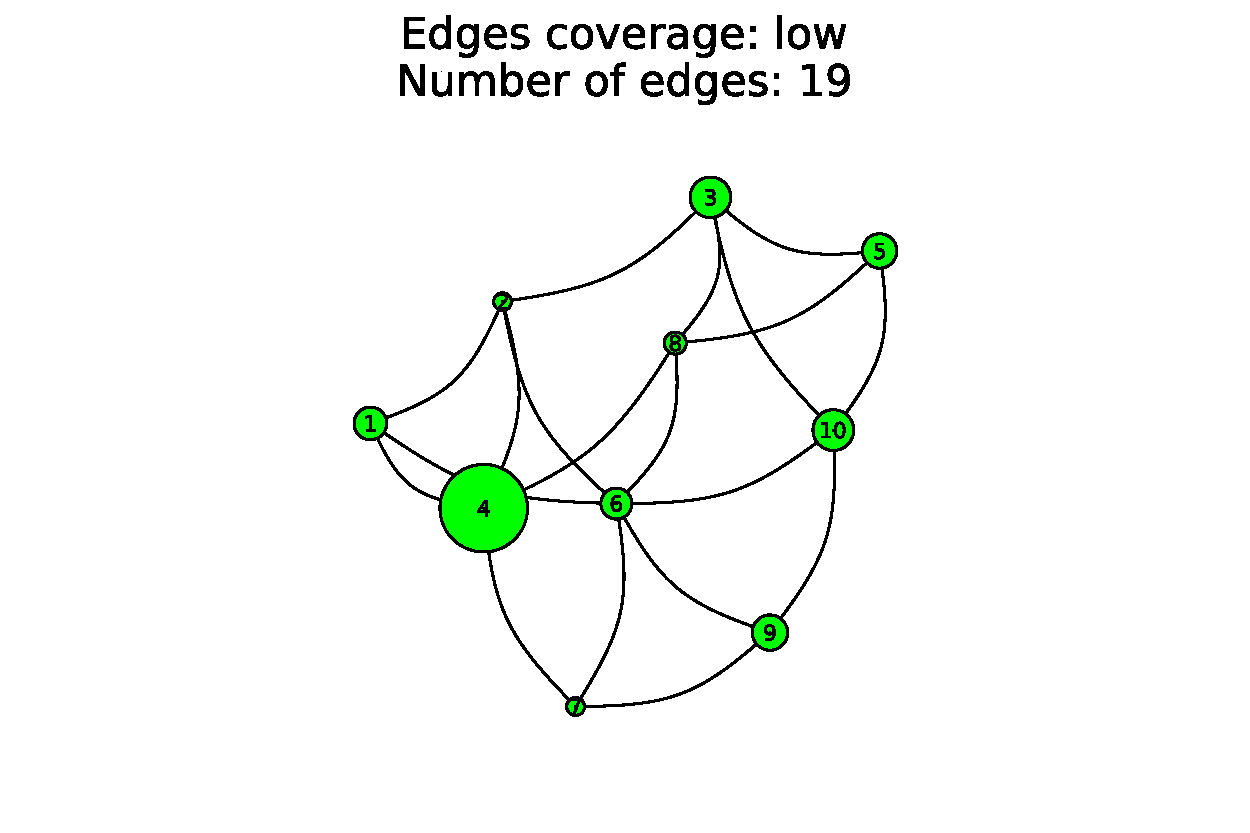
\includegraphics[width=\textwidth]{img/low.pdf}
		\caption{Esempio di grafo connesso con copertura bassa}
		\label{fig:connected_graph_example_low}
	\end{subfigure}
	\hfill
	\begin{subfigure}[b]{0.3\textwidth}
		\centering
		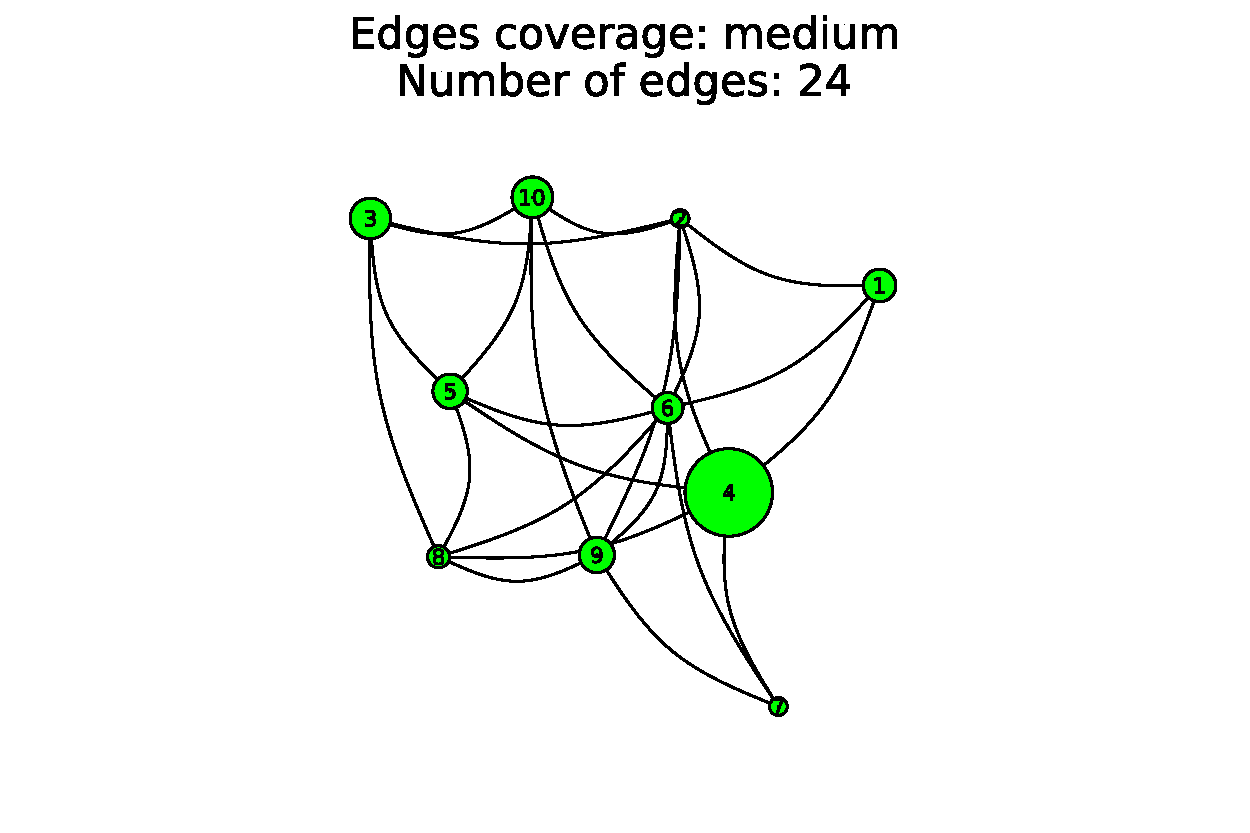
\includegraphics[width=\textwidth]{img/medium.pdf}
		\caption{Esempio di grafo connesso con copertura media}
		\label{fig:connected_graph_example_medium}
	\end{subfigure}
	\hfill
	\begin{subfigure}[b]{0.3\textwidth}
		\centering
		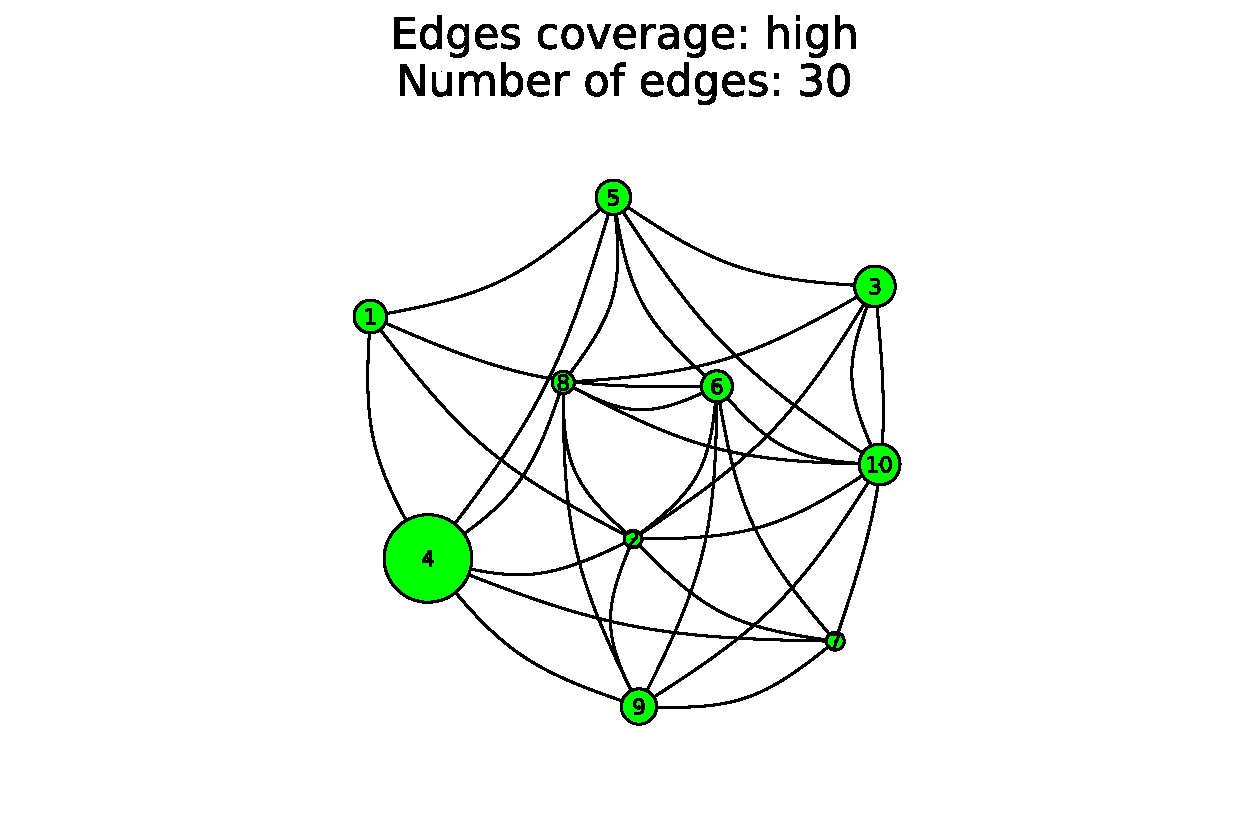
\includegraphics[width=\textwidth]{img/high.pdf}
		\caption{Esempio di grafo connesso con copertura alta}
		\label{fig:connected_graph_example_high}
	\end{subfigure}
\end{figure}

Con questo approccio la modellazione del problema e soprattutto la dinamica intera del 
modello verte più su un approccio di tipo \emph{mesoscopico} tendente al \emph{macroscopico}.
Questo poichè per quanto l'idea di modellare un sistema ad agente estremamente granulare fosse 
di non poco interesse, al lato pratico ci si sarebbe scontrati con delle difficoltà 
intrinseche ad una modellazione così specifica, la quale non si adattava all'idea più 
ampia del problema. Difatti non si vuole modellare un sistema a livello microscopico per vedere
le possibili interazioni tra agenti differenti, bensì si vuole vedere la risposta collettiva di un
agente astratto all'utilizzo di interventi mirati e specifici per contrastare l'epidemia in 
maniera localizzata.

\subsection{Approccio con Rete Sociale}
Il modello utilizzato sfrutta le proprietà del framework \textbf{Agents.jl} e definisce un 
modello ad agente di tipo \textbf{ABM}. Essendo che in questo caso la struttura spaziale 
del modello non è importante ma le sue connessioni si, vengono definiti gli agenti come nodi
veri e propri del grafo in cui al loro interno viene simulato il ciclo di vita della pandemia 
tramite un modello di tipo \textbf{SEIR} deterministico.

La struttura dell'agente è di tipo \textbf{ContinuousAgent} in quanto lo 
spazio del modello è di tipo continuo. Questa scelta è stata fatta in vista di possibili 
sviluppi futuri dell'applicazione. Successivamente si può osservare come il modello generato 
in figura \ref{fig:Model_code} sia molto snello, avendo solamente una manciata di parametri 
sufficienti al corretto funzionamento del modello stesso. 

\subsubsection*{Grafo sociale}
Un grafo sociale è un particolare tipo di grafo che rappresenta le relazioni sociali tra entità.
Questo approccio viene largamente utilizzato per la rappresentazione delle reti sociali dove la 
parola \emph{grafo} viene presa dalla teoria dei grafi. Generalmente un grafo sociale viene riferito come un
grafo che mappa gli individui come nodi e le loro relazioni come archi. \cite{wiki:Social_graph}

\begin{minipage}{\linewidth}
    \centering
    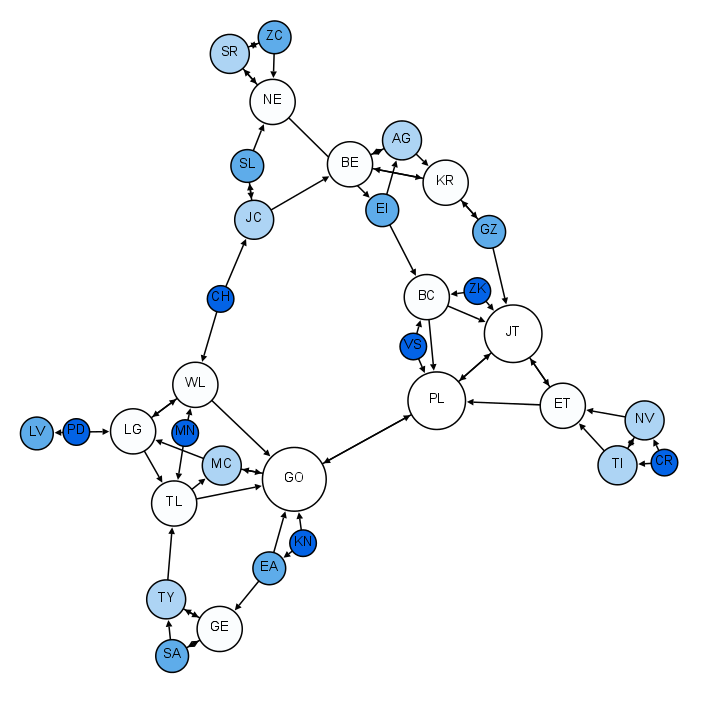
\includegraphics[width=\textwidth]{img/Moreno_Sociogram_3rd_Grade.png}
    \captionof{figure}{Esempio di grafo sociale}
    \label{fig:social_graph}
\end{minipage}

Il concetto è stato originariamente coniato dalla struttura dati \textbf{sociogramma} \cite{wiki:Sociogram}, 
una struttura a grafo che rappresenta i collegamenti sociali che hanno gli individui da esso modellato, ovvero le persone. 
Questa struttura dati si occupa di stutturare le relazioni interpersonali che si formano all'interno di un 
gruppo di individui. 

\subsubsection{Agente}

\begin{minipage}{\linewidth}
    \centering
    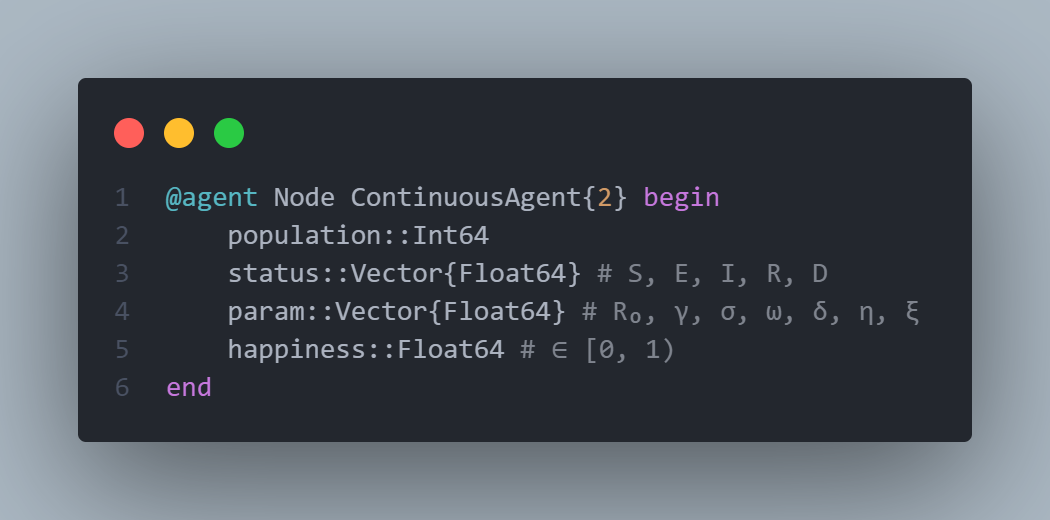
\includegraphics[width=\textwidth]{img/node_agent.png}
    \captionof{figure}{Codice Agente}
    \label{fig:Agent_code}
\end{minipage}

Come mostrato in figura \ref{fig:Agent_code} l'agente al suo interno è molto minimale,
descrivendo solamente gli attributi necessari e sufficienti per la corretta modellazione
e interazione con l'ambiente, il modello e gli altri agenti, e se stesso. L'evoluzione di 
ogni agente è completamente indipendente dall'evoluzione degli altri, ma può essere influenzata da 
altri agenti della rete, modificando l'altrimenti determinismo del modello SEIR al suo interno. 

I campi principali dell'agente sono i seguenti:
\begin{itemize}
	\item \textbf{population}: questo campo descrive tramite un valore di tipo \textbf{Int}
	il numero totale di individui che ad ogni step del modello si trovano all'interno di uno 
	specifico nodo. 
	\item \textbf{status}: questo campo descrive tramite un vettore di tipo \textbf{Float64}
	lo stato della popolazione all'interno del nodo. Questo stato viene descritto come 
	percentuale di individui, per cui i valori all'interno del vettore saranno tutti compresi 
	tra 0 e 1. La scelta di utilizzare questo approccio è nata principalmente per motivi di 
	\emph{type stability} in quanto le operazioni di risoluzione del sistema di ODE altrimenti 
	potrebbero risentirne. Tuttavia è stato fatto anche per un fattore di \emph{facilità di comprensione}.
	\item \textbf{param}: questo campo descrive tramite un vettore di tipo \textbf{Float64}
	i parametri del modello SEIR specifici del nodo in questione. Questi parametri sono comprensivi 
	non solo dei valori relativi all'epidemia, ma anche dei valori relativi alle contromisure, 
	in particolare le contromisure \textbf{non farmaceutiche} rappresentate dal valore \textbf{$\eta$}
	e quelle \textbf{farmaceutiche} rappresentate dal valore \textbf{$\xi$}.
	\item \textbf{happiness}: questo campo è utilizzato come campo di appoggio per il bilanciamento
	delle contromisure applicate dal controllore.
\end{itemize}

\subsubsection{Spazio e Modello}

\begin{minipage}{\linewidth}
    \centering
    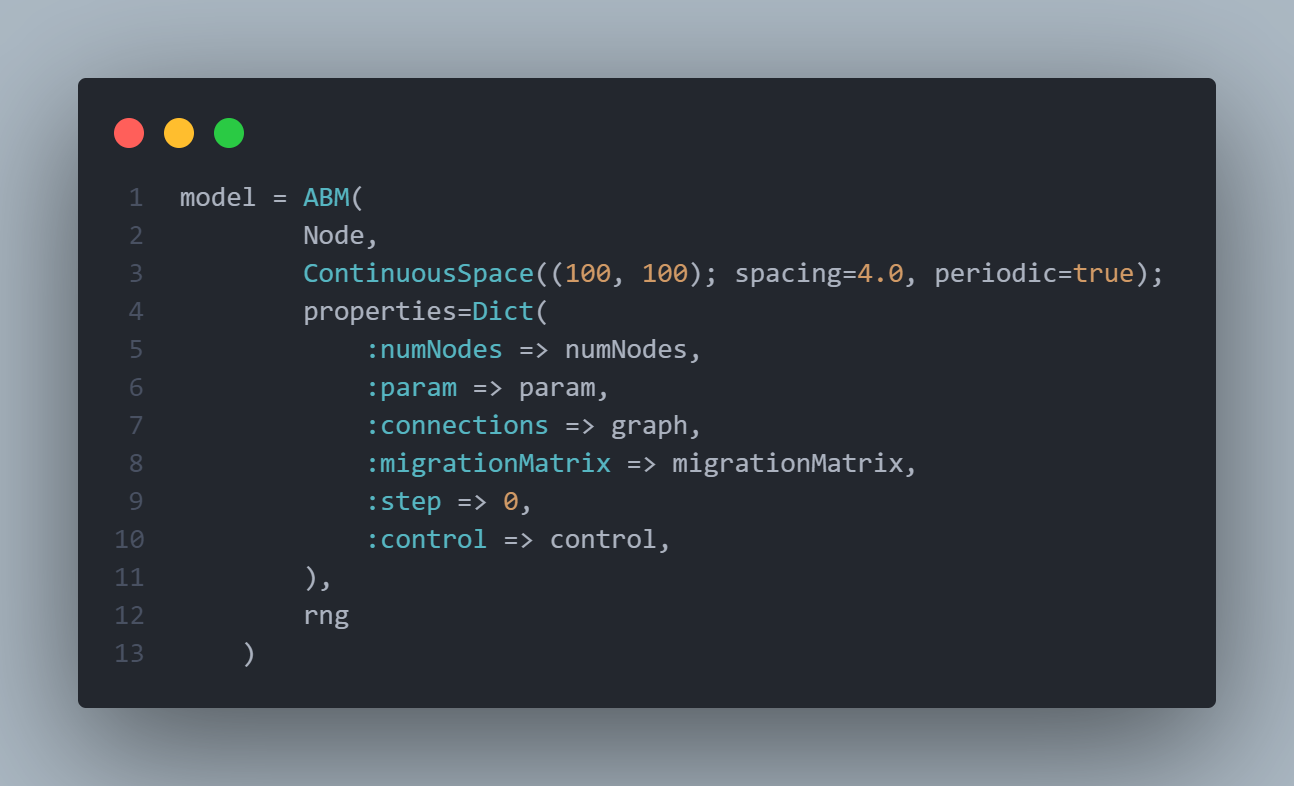
\includegraphics[width=\textwidth]{img/sngraph_model.png}
    \captionof{figure}{Codice Modello}
    \label{fig:Model_code}
\end{minipage}

Come accennato precedentemente e mostrato in figura \ref{fig:Model_code}, lo spazio del modello 
è di tipo \textbf{ContinuousSpace} seppure non venga effettivamente sfruttato a dovere. 
Tuttavia l'interesse del modello è il fatto che utilizzi una struttura come un grafo in maniera
astratta per modellare le interazioni tra i suoi nodi, ovvero gli agenti, in maniera rapida ed efficente.

Per prima cosa viene creato il modello tramite la creazione di un grafo \emph{connesso}, il cui 
numero di archi dipende da quanto l'utente vuole che siano connessi i nodi. Più alto è il 
desiderio di copertura più archi verranno creati. Tuttavia ci sono dei limiti superiori e inferiori 
sul numero di nodi creabili.

\begin{figure}[!hb]
	\centering
	\begin{subfigure}[b]{0.45\textwidth}
		\centering
		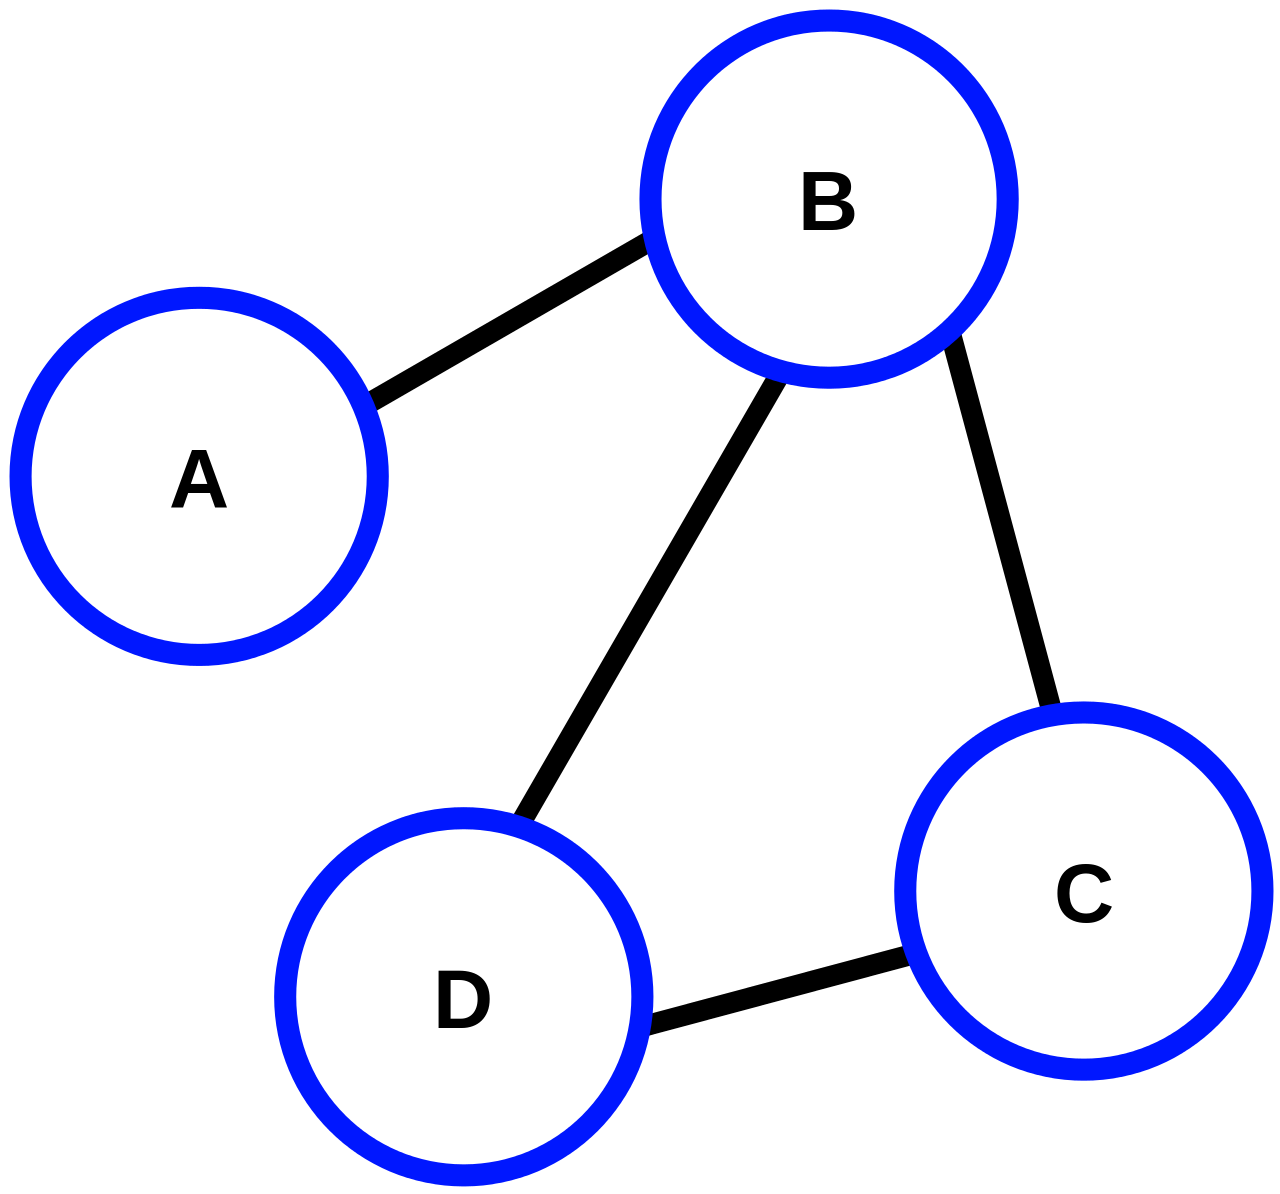
\includegraphics[width=\textwidth]{img/CPT-Graphs-undirected-unweighted-ex1.svg.png}
		\caption{Esempio di grafo connesso}
		\label{fig:connected_graph_example}
	\end{subfigure}
	\hfill
	\begin{subfigure}[b]{0.45\textwidth}
		\centering
		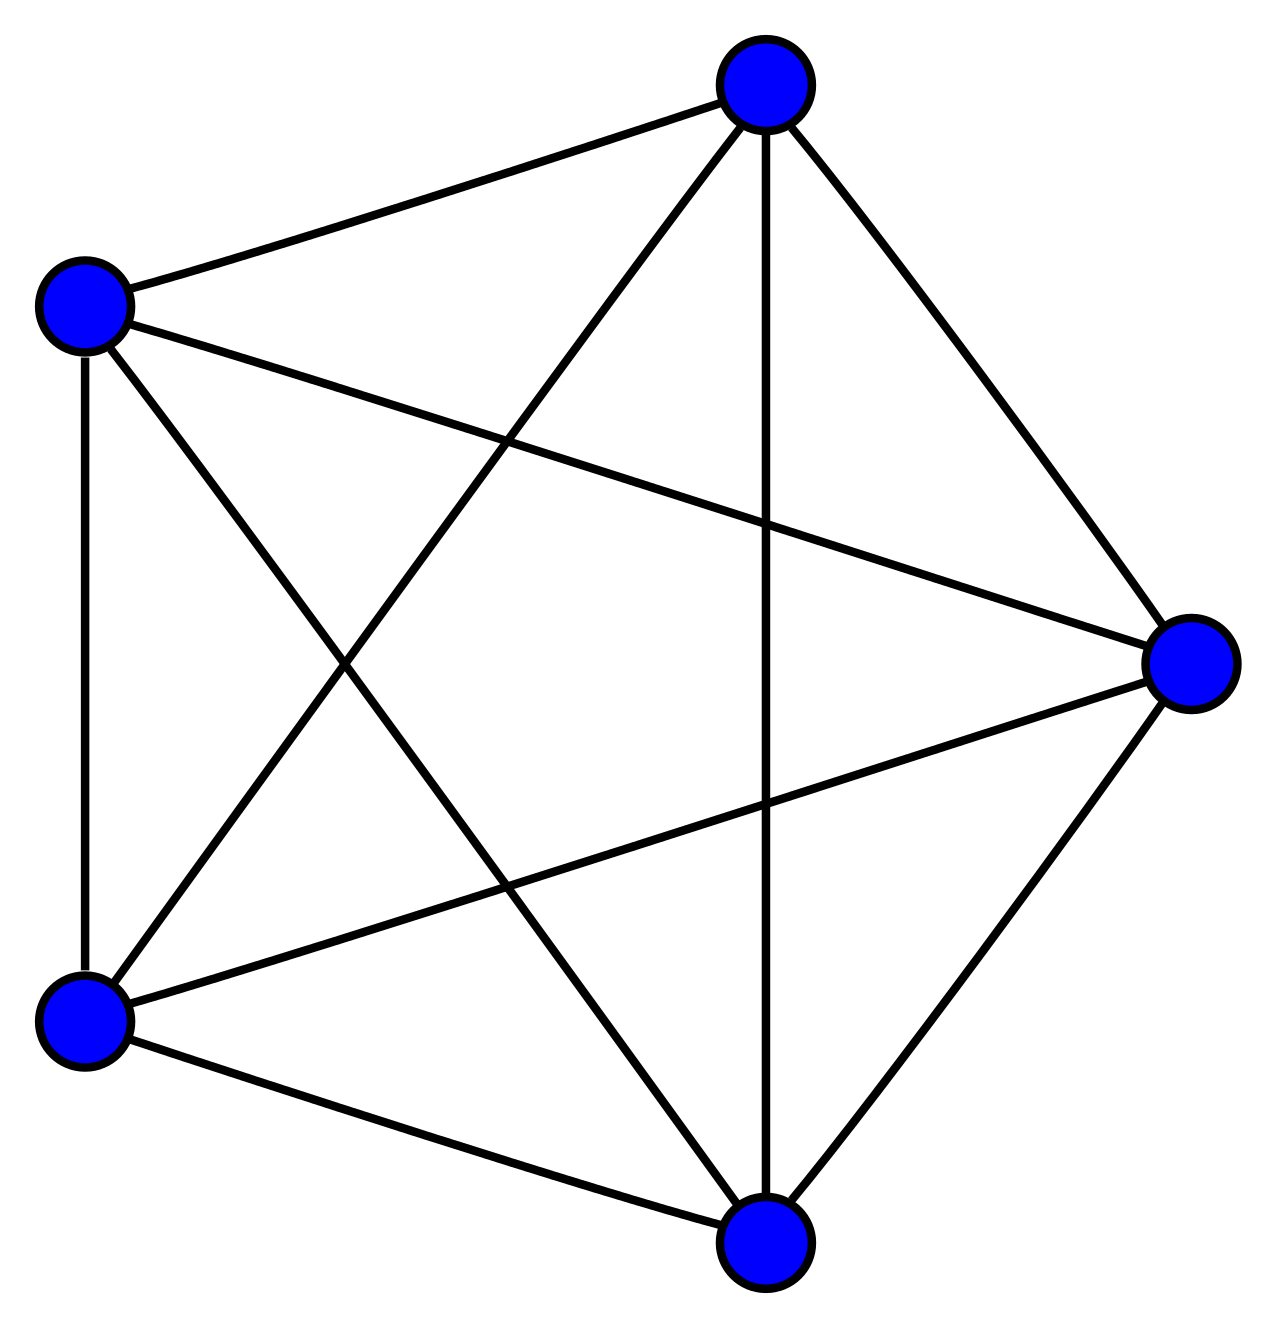
\includegraphics[width=\textwidth]{img/4-simplex_graph.svg.png}
		\caption{Esempio di grafo completo}
		\label{fig:complete_graph_example}
	\end{subfigure}
\end{figure}

Il grafo che si va a creare è \emph{non orientato}, per cui il numero minimo di archi necessari 
per costruire un grafo connesso, ovvero un grafo in cui da ogni nodo è sempre possibile raggiungere
tutti gli altri nodi tramite un percorso che li collega, diventa il segunte: $numEdges = numNodes-1$
e questo pone il limite inferiore. Quello superiore è dato dalla costruzione di un grafo completo, 
un grafo per cui ogni nodo è collegato con tutti gli altri nodi appartenenti al grafo. In questo 
caso il numero di archi necessari è: $numEdges = \frac{numNodes*(numNodes-1)}{2}$.

All'interno di questi due limiti, viene creato il grafo secondo le esigenze dell'utente come mostrato 
in figura \ref{fig:graph_coverage}. Successivamente viene creata una matrice di flusso, denominata 
\textbf{migrationMatrix} che rappresenta la percentuale di individui che dal nodo di interesse 
si spostano verso un nodo obiettivo. Questa matrice è salvata come \textbf{matrice sparsa} per 
risparmiare spazio dove le connessione non sono presenti tra i nodi. 

\begin{minipage}{\linewidth}
	\centering
	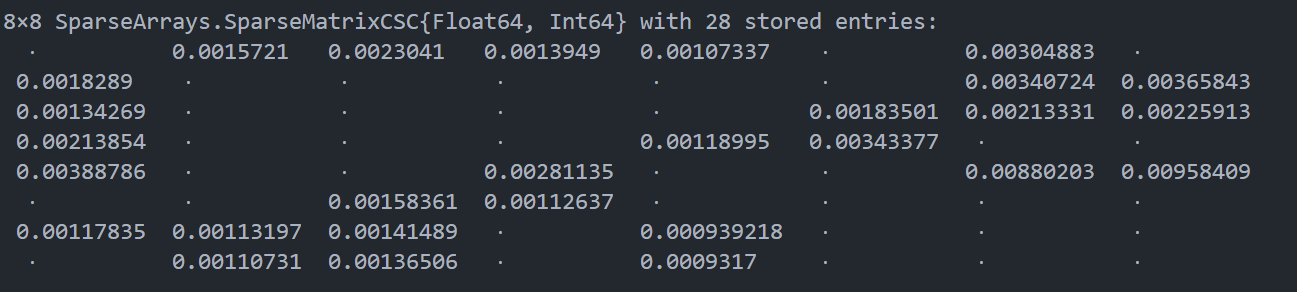
\includegraphics[width=\textwidth]{img/migrationMatrix.png}
	\captionof{figure}{Matrice di migrazione dato un MigrationRate di 0.01}
	\label{fig:migration matrix}
\end{minipage}

Questa matrice viene esplicitamente creata in base alla topologia del grafo che viene 
inizializzato in precedenza e si occupa di pesare gli archi di quest'ultimo seguendo la 
filosofia per cui si ha un flusso maggiore verso i nodi più popolosi, e minore verso i 
nodi meno popolosi. 

\begin{minipage}{\linewidth}
	\centering
	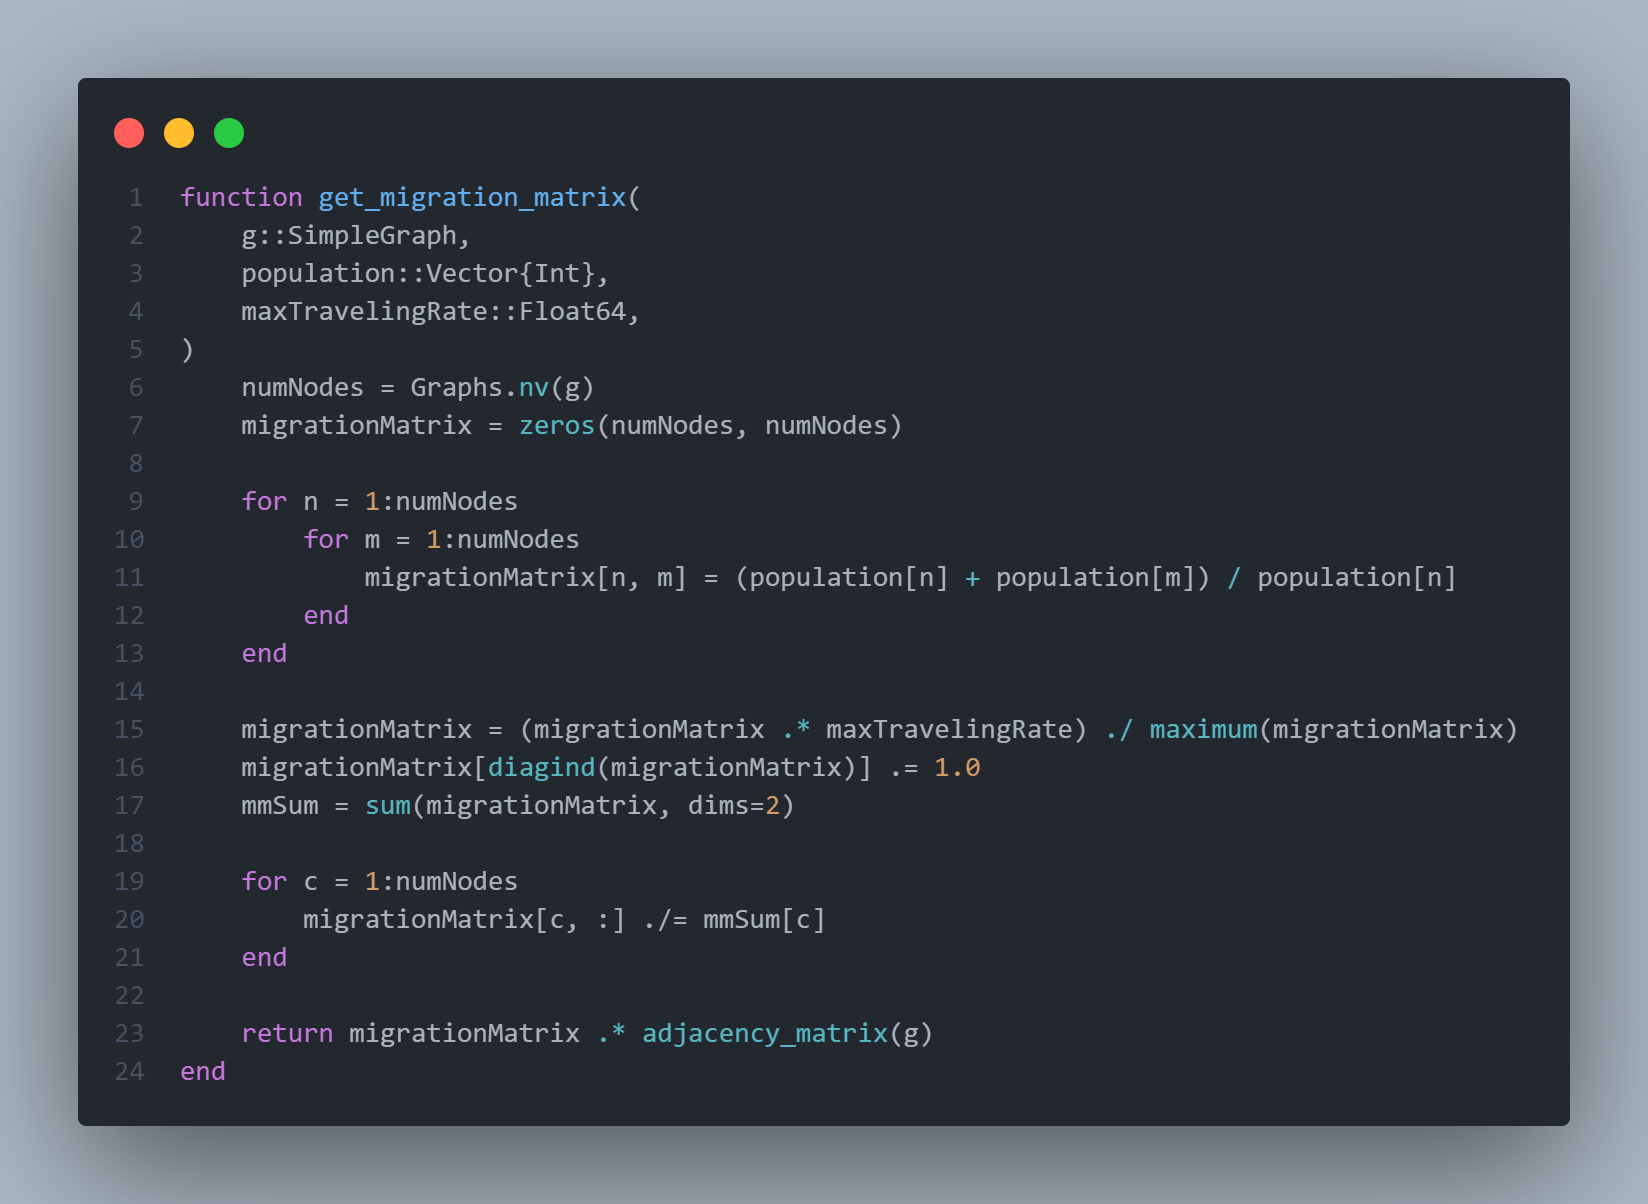
\includegraphics[width=\textwidth]{img/mmfunc.png}
	\captionof{figure}{Funzione che crea la matrice di migrazione data la topologia di un grafo}
	\label{fig:migration_matrix_function}
\end{minipage}

Se questa matrice fosse una matrice non sparsa, e perciò completa, si potrebbe osservare
come la diagonale di questa matrice ha valori molto vicini ad 1, in relazione con il limite
massimo di individui che possono migrare da ogni nodo, definito come \emph{migration rate}; 
andando a delineare come la maggior parte della popolazione non effettui in genere spostamenti 
tra nodi ma che sia più probabile che rimanga nel suo nodo di origine. Questa assunzione può 
variare nel tempo ad esempio nei periodi di alto flusso migratorio come ad esempio i periodi 
estivi o più in generale i periodi strettamente collegati alle vacanze.

Successivamente, dopo avere popolato ogni agente (o nodo) del modello con i corretti valori,
dato che la struttura interna su cui viene effettuata la computazione del modello è basata su 
un sistema di ODE, viene istanziato un array di \textbf{ODEProblem}. L'idea di spezzettare
un sistema di ODE in più sottosistemi di ODE collegate tra loro tramite uno scambio continuo 
di informazioni (in questo caso individui), è stata pubblicata nel seguente articolo \cite{Ding2021}
in cui si modella l'outbreak da COVID-19 tenendo in considerazione il flusso migratorio 
dei voli aerei da e verso differenti nazioni. 

Applicando tale filosofia, è possibile creare un array di \textbf{ODEProblem}, oggetti che descrivono
un sistema di equazioni differenziali ordinarie, ai quali viene messo a corredo un \textbf{integratore}. 
Quest'ultimo fa le veci della classica funzione \textbf{solve} che si occupa di risolvere l'intero sistema.

\begin{minipage}{\linewidth}
	\centering
	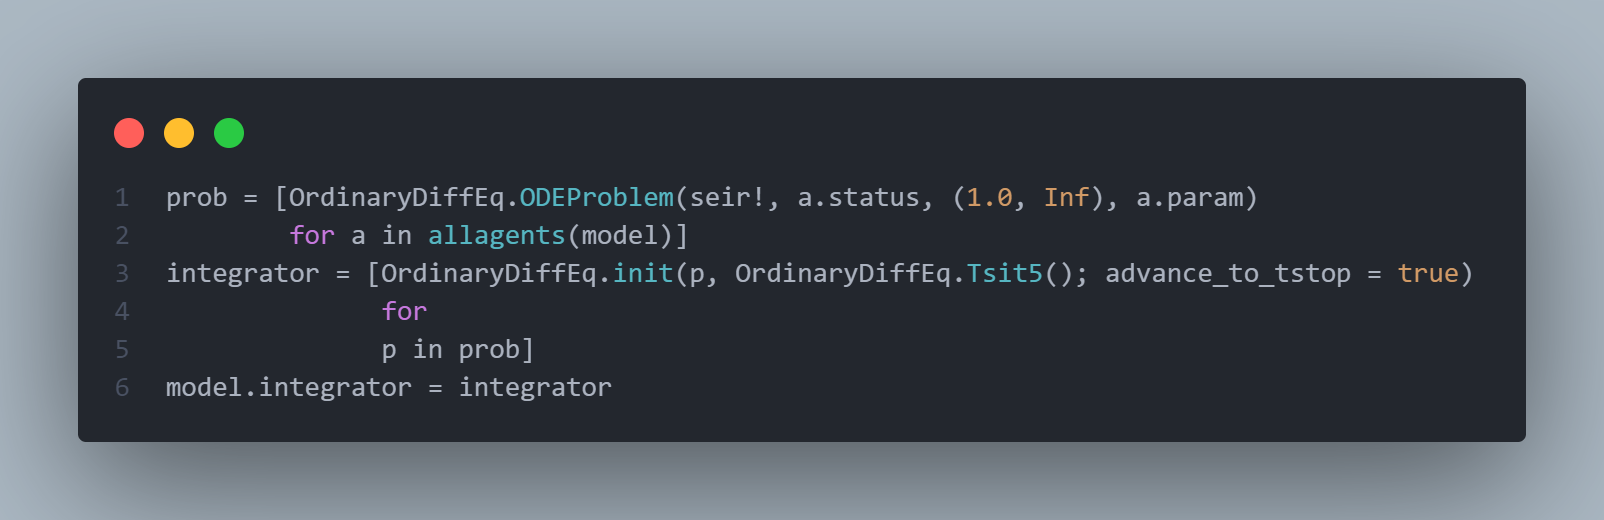
\includegraphics[width=\textwidth]{img/model_ode.png}
	\captionof{figure}{Definizione dei sistemi di ODE associati ad ogni agente}
	\label{fig:model_ode}
\end{minipage}

L'approccio scelto, ovvero di usare un integratore, può essere sostituito tramite
l'uso di funzioni di \textbf{callback} le quali permettono quando vengono soddisfatte delle
condizioni di attivazione specifiche, di andare a modificare i parametri del sistema che
si sta risolvendo. Queste modifiche tuttavia, possono portare delle discontinuità nella 
risoluzione, ma queste vengono esplicitamente gestite se viene specificata una funzione 
di callback all'interno della funzione di solve, altrimenti l'integratore deve essere notificato che 
i parametri e i valori al suo interno possono essere stati modificati. 

I due approcci sono completamente equivalenti e la scelta di uno piuttosto che dell'altro
ricade solamente su un fattore di comodità d'uso.

\subsubsection{Funzione di avanzamento agente}
Un agente finchè all'interno di un modello segue ciclicamente il comportamento
riportato in figura \ref{fig:agent_behaviour}

\begin{minipage}{\linewidth}
	\centering
	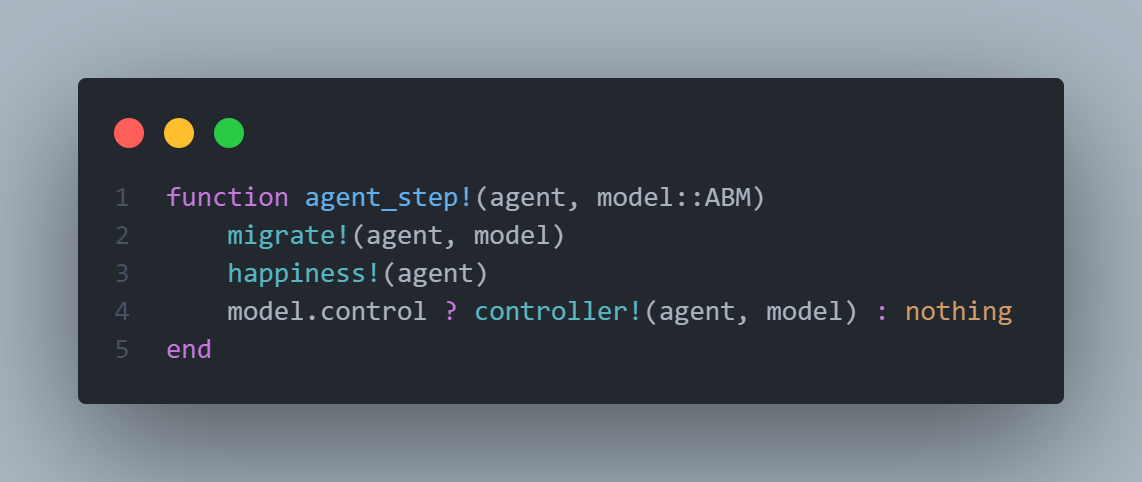
\includegraphics[width=\textwidth]{img/agent_behaviour.png}
	\captionof{figure}{Comportamento agente}
	\label{fig:agent_behaviour}
\end{minipage}

Ad ogni passo del modello, vengono attivati tutti gli agenti presenti al suo interno e 
fatti aggiornare seguendo le regole di scheduling preposte. 

Ad ogni passo, un agente è chiamato ad eseguire tre fondamentali compiti:
\begin{itemize}
	\item \textbf{Muoversi}: un agente come entità essendo un nodo di un grafo non può
	muoversi nel modo più letterale del termine, ma tramite la sua matrice di migrazione 
	è possibile calcolare quanti individui si spostano da il nodo sorgente, fino ad un nodo
	destinazione. Questo spostamento fa si che il nodo venga aggiornato con le relative percentuali
	di status e il totale di popolazione rimanente

	\begin{minipage}{\linewidth}
		\centering
		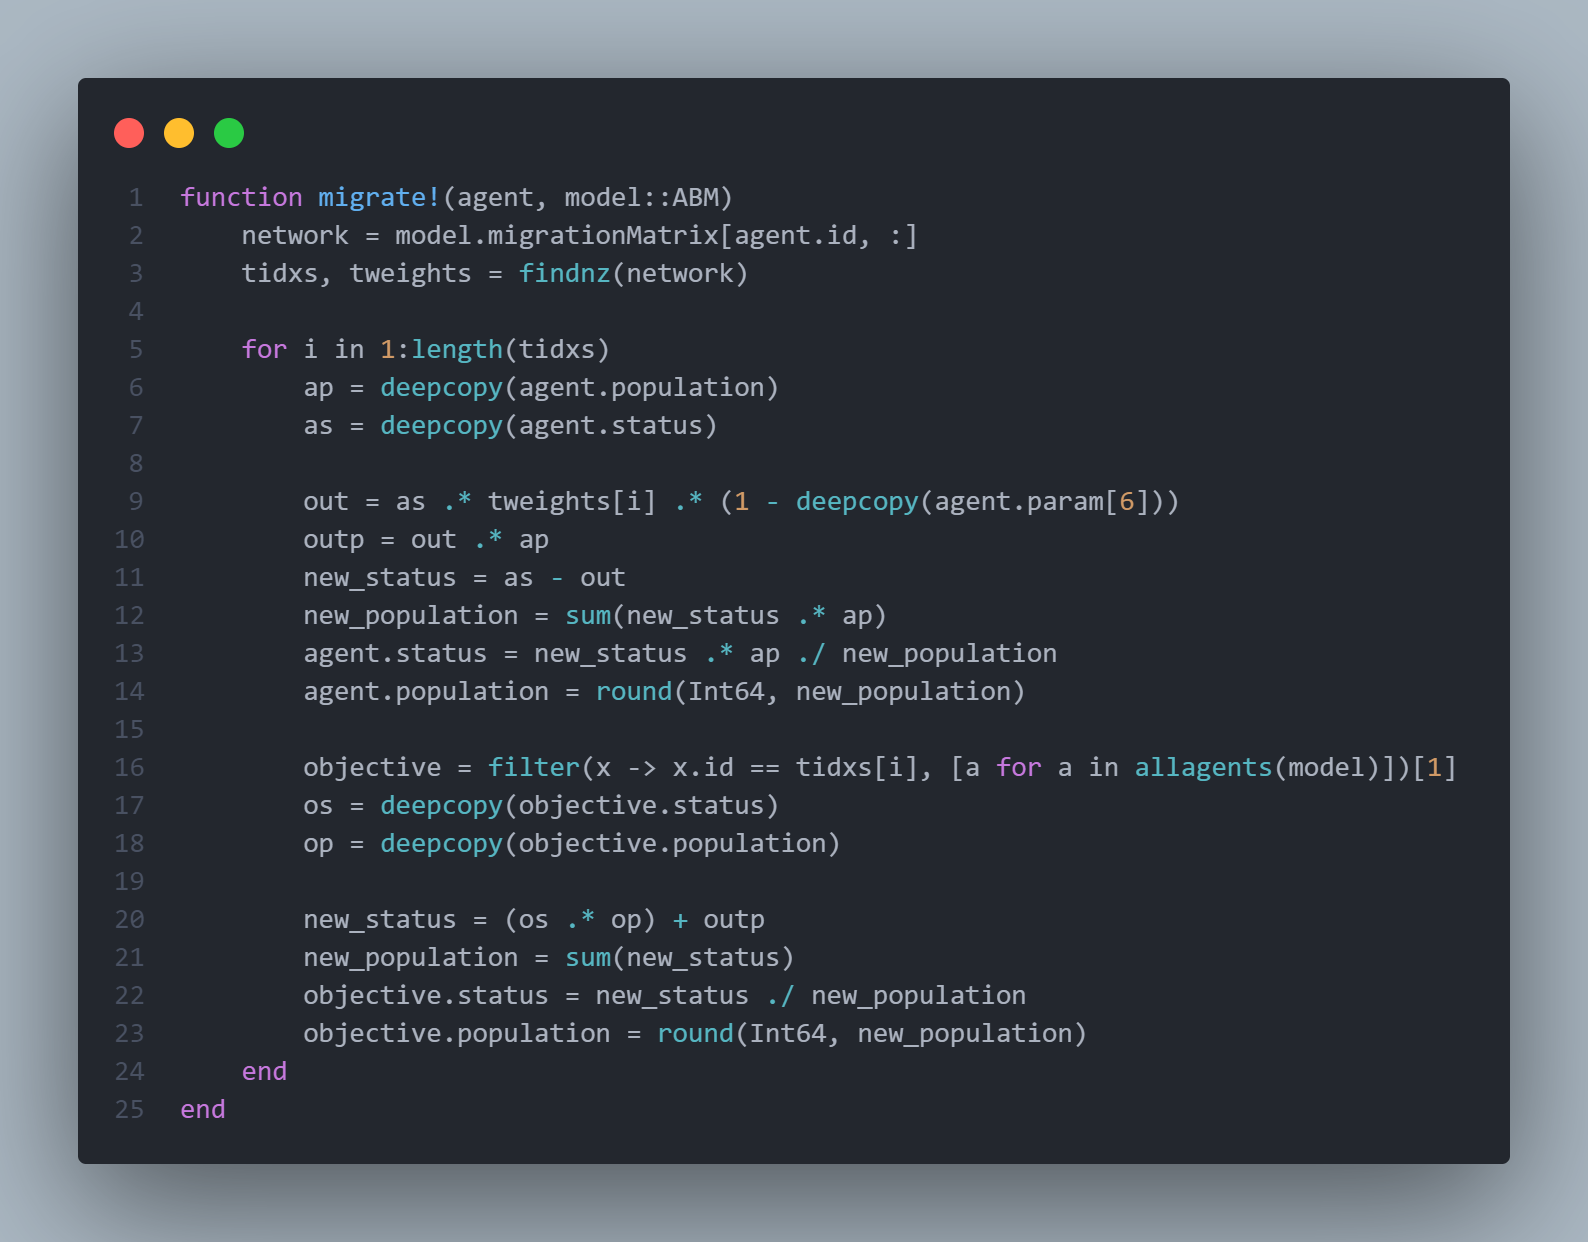
\includegraphics[width=\textwidth]{img/migratef.png}
		\captionof{figure}{Funzione atta a calcolare lo spostamento di agenti da un nodo all'altro del grafo}
		\label{fig:migrationf}
	\end{minipage}

	\item \textbf{Calcolare la felicità}: come detto in apertura della sezione, il valore di \textbf{happiness}
	è un valore fantoccio che serve prevalentemente per bilanciare le contromisure del controllore.
	Questo valore tuttavia viene influenzato anche dalla situazione pandemica. 
	
	\begin{minipage}{\linewidth}
		\centering
		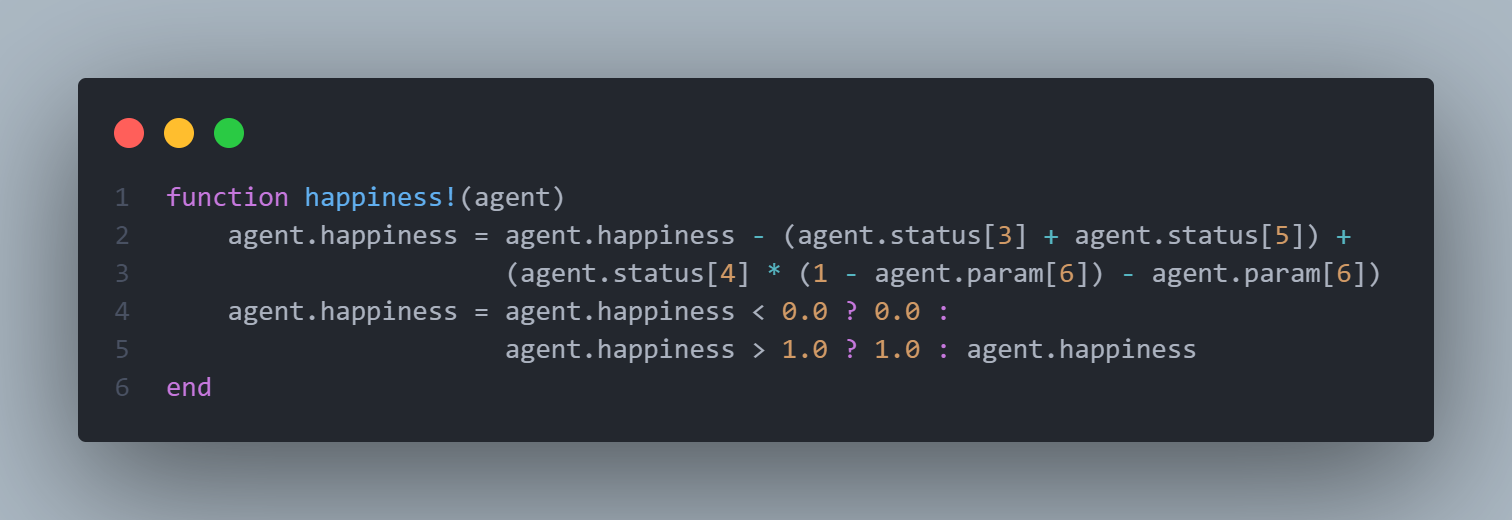
\includegraphics[width=\textwidth]{img/happiness.png}
		\captionof{figure}{Funzione atta a calcolare la felicità degli agenti}
		\label{fig:happinessf}
	\end{minipage}

	Questo approccio è sicuramente problematico e fallace per numerosi motivi ma attualmente 
	adempie al suo obiettivo di gestore del controllore, in quanto non è mai stato inteso di 
	realizzare uno stimatore affidabile per l'umore generele di una popolazione durante una situazione
	estrema come può essere una pandemia.
	\item \textbf{Chiamare il controllore}: se la proprietà \emph{control} del modello è impostata su
	\emph{true}, viene chiamato il controllore che si occupa di stimare, data la situazione attuale del nodo
	quanto stringenti devono essere le policy da applicare al nodo in questione per cercare di minimizzare il 
	numero di infetti in un determinato numero di passi. 
\end{itemize}

\subsubsection{Funzione di avanzamento modello}
Ogni passo di avanzamento del modello segna un passo di avanzamento dell'intero sistema. 
Questo vuol dire che all'interno di un passo del modello vi è un passo per ogni agente. Di default
il framework Agents.jl effettua prima l'avanzamento degli agenti e successivamente quello del modello.
Questo comportamento può essere modificato quando viene chiamata la funzione di \textbf{step!} che 
si occupa di far girare l'intero sistema.

Il modello si occupa ad ogni passo di effettuare tutte quelle operazioni che non sono legate ad un
singolo agente ma che sono legate o alla comunità di agenti oppure al modello in quanto sistema complesso. 

\begin{minipage}{\linewidth}
	\centering
	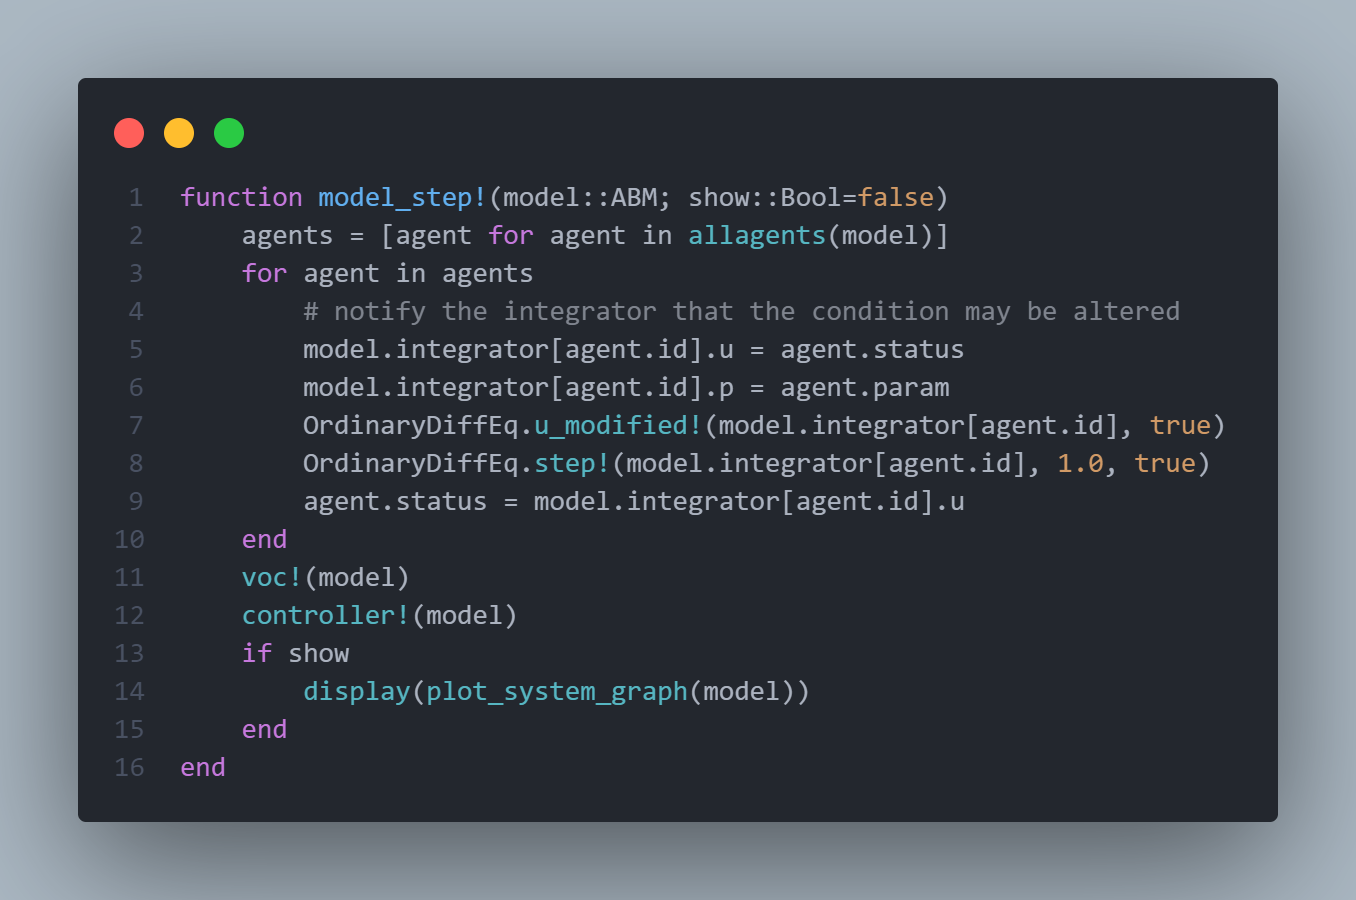
\includegraphics[width=\textwidth]{img/model_step.png}
	\captionof{figure}{Funzione di avanzamento del modello}
	\label{fig:model_step}
\end{minipage}

Come è possibile osservare dalla figura \ref{fig:model_step}, il sistema si occupa principalmente
di aggiornare notificare l'integratore di ogni agente e aggiornarlo indicandogli che le condizioni
precedenti possono essere state alterate, e successivamente effettuare un passo del sistema di 
integrazione. Successivamente il modello si preoccupa di generare una nuova \emph{\textbf{V}ariant \textbf{O}f \textbf{C}oncern} (VOC)
e infine di chiamare la funzione \textbf{vaccine!} la quale è responsabile del calcolo e dell'applicazione 
delle misure di contromisure farmaceutiche all'interno della popolazione. 

Questa sezione è quella che più presta il fianco ad \emph{assunzioni} riguardo 
il comportamento generale del sistema. Tutte le funzioni sopra descritte si basano su un insieme
più o meno nutrito di assunzioni per funzionare correttamente. 
La funzione che si occupa di generare la VOC è la seguente

\begin{minipage}{\linewidth}
	\centering
	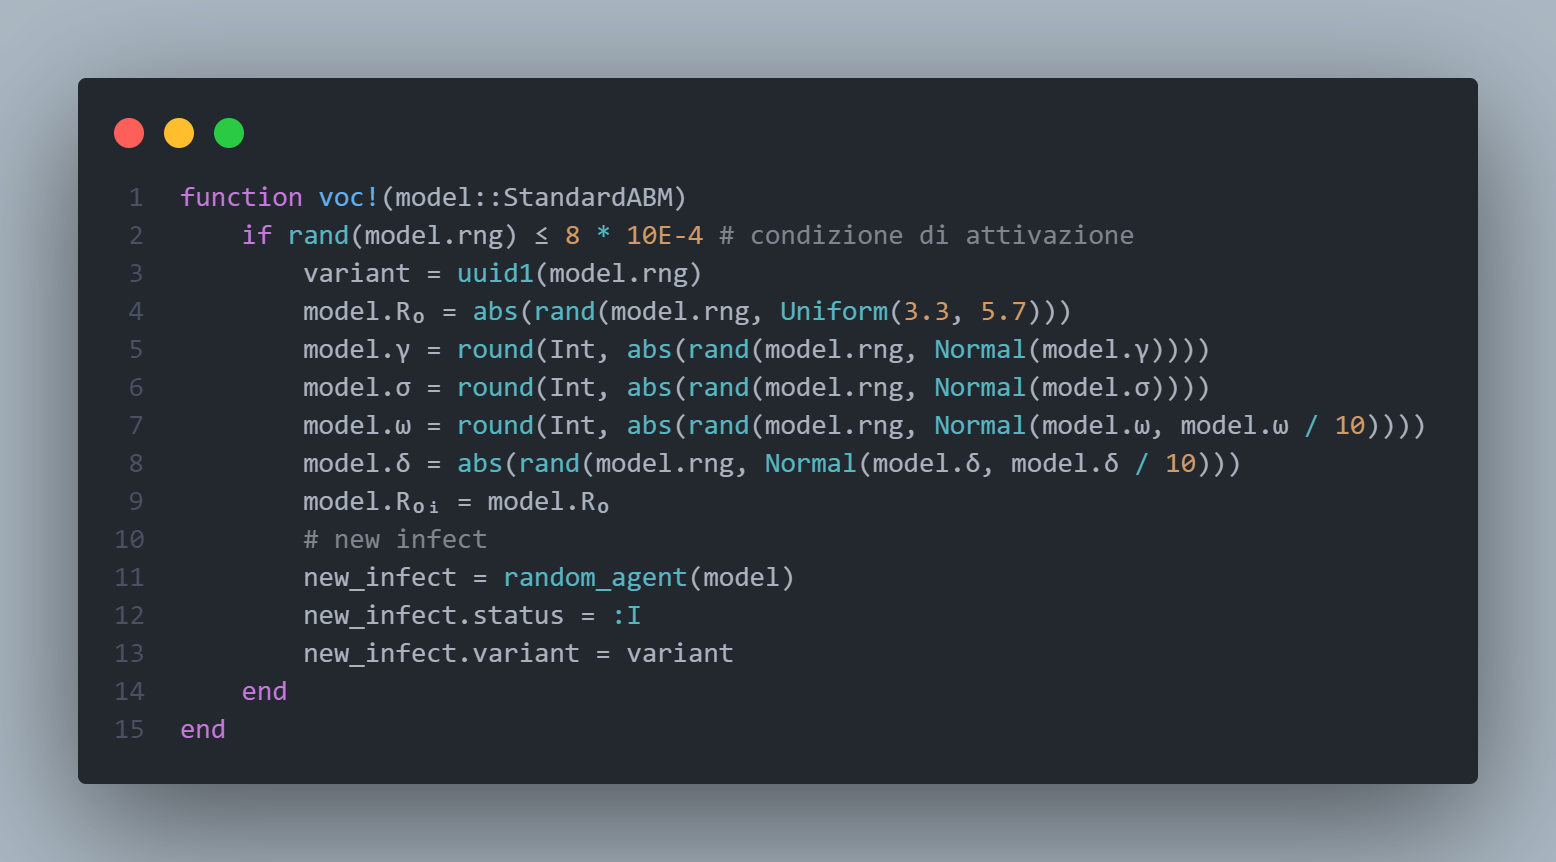
\includegraphics[width=\textwidth]{img/voc.png}
	\captionof{figure}{Funzione che si occupa di generare la VOC}
	\label{fig:voc}
\end{minipage}

Si possono notare molte assunzioni:
\begin{itemize}
	\item la condizione di attivazione della funzione si basa su un valore
	che sembra totalmente randomico. Quel valore, ovvero $8e-3$ deriva dai
	seguenti articoli \cite{Markov2023} \cite{https://doi.org/10.1002/jmv.27331} \cite{Abavisani2022}
	i quali descrivono prevalentemente il tasso di mutazione casuale delle basi che compongono
	il DNA del virus SARS-COV2. Questo però non implica che tali mutazioni 
	creino una VOC. Per semplicità è stato scelto di usare l'approccio per cui
	se una mutazione avviene, questa è un a VOC e, in linea di massima, sembra che 
	questo approccio semplicistico descriva un numero di VOC generalmente sensato e 
	in linea con quanto abbiamo potuto osservare durante la pandemia, facendo ipotizzare che 
	la scelta di usare uno stimatore così semplicistico possa comunque portare a dei benefici
	\item la distribuzione dei parametri associati alla pandemia viene calcolata
	seguendo una distribuzione \textbf{Normale}, tranne per la distribuzione dell'indice $R_0$
	il quale segue una distribuzione di tipo \textbf{Uniforme} \cite{wiki:Numero_di_riproduzione_di_base}.
	Questa scelta non ha alcun riscontro in letteratura in quanto non vi sono studi 
	che attestano in che modo una variante influenzi i parametri stessi del virus, 
	tanto meno se questa influenza si distribuisce seguendo un andamento normale. 
	Ciò nonostante questa brutale semplificazione è stata applicata per dare un senso 
	all'altrimenti insensata implementazione di una variante.
\end{itemize}

La funzione che si occupa di stimare l'applicazione delle contromisure farmaceutiche, 
ovvero l'applicazione del vaccino, è la seguente, e anch'essa presta il fianco 
a numerevoli assunzioni, le quali però empiricamente parlando
effettuano una buona stima di come sono evolute le cose nel mondo reale.

\begin{minipage}{\linewidth}
	\centering
	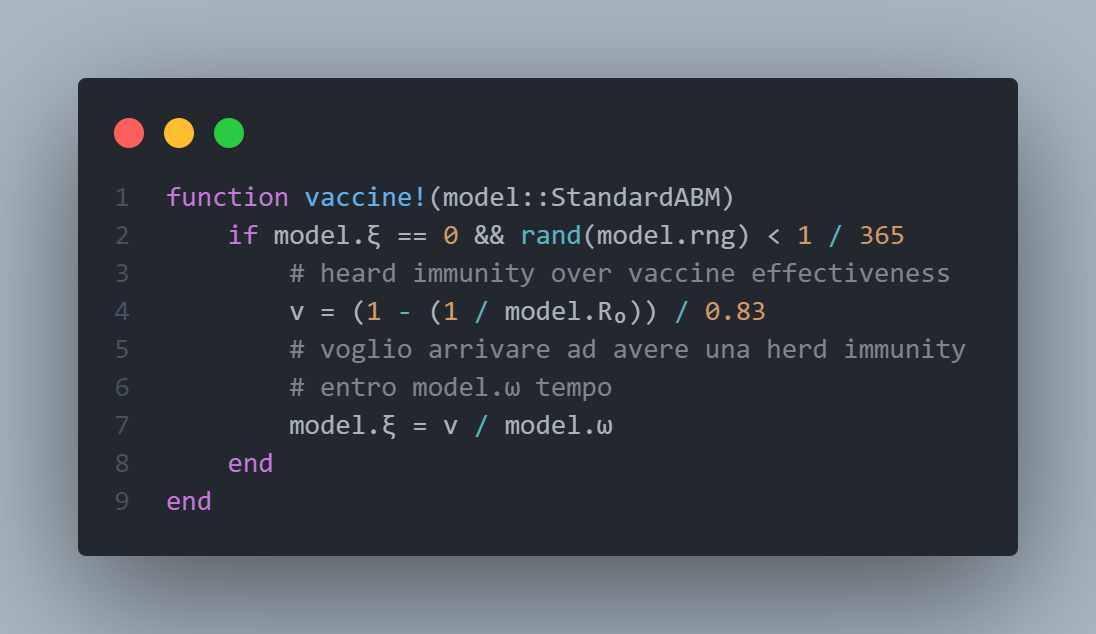
\includegraphics[width=\textwidth]{img/vaccine.png}
	\captionof{figure}{Funzione che si occupa di simulare la ricerca di un vaccino e la sua successiva applicazoine}
	\label{fig:vaccine}
\end{minipage}

Si nota come in generale la funzione si basa sul generare un valore fissato, 
generalmente $\in [0,1]$, che rappresenta la percentuale di popolazione che può 
essere vaccinata ad ogni passo del modello. Questo approccio tende a simulare l'idea 
più o meno realistica di avere una quantità fissata di dosi vaccinali 
ogni giorno che possono essere erogate alla popolazione. 

Questo calcolo viene effettuato tenendo in considerazione l'approccio 
dell' \emph{immunità vaccinale di gregge} \cite{wiki:Immunità_di_gregge} 
che può essere ottenuta seguendo la formula 

$$V_c = \frac{1-\frac{1}{R_0}}{VaccineEfficiency}$$

Successivamente calcolo questo valore come un obiettivo da raggiungere entro un tempo $\omega$ 
che equivale al periodo di immunità che un individuo ha dopo aver contratto la malattia 
(o aver effettuato il vaccino). Questa idea viene utilizzata per modellare le curve del 
modello in quanto un individuo vaccinato è considerato come un individuo nello stato 
\emph{Recovered} e segue le stesse regole di chiunque altro, indipendentemente
dal modo in cui si è entrati in questo stato. 

\begin{figure}[!hb]
	\centering
	\begin{subfigure}[b]{0.45\textwidth}
		\centering
		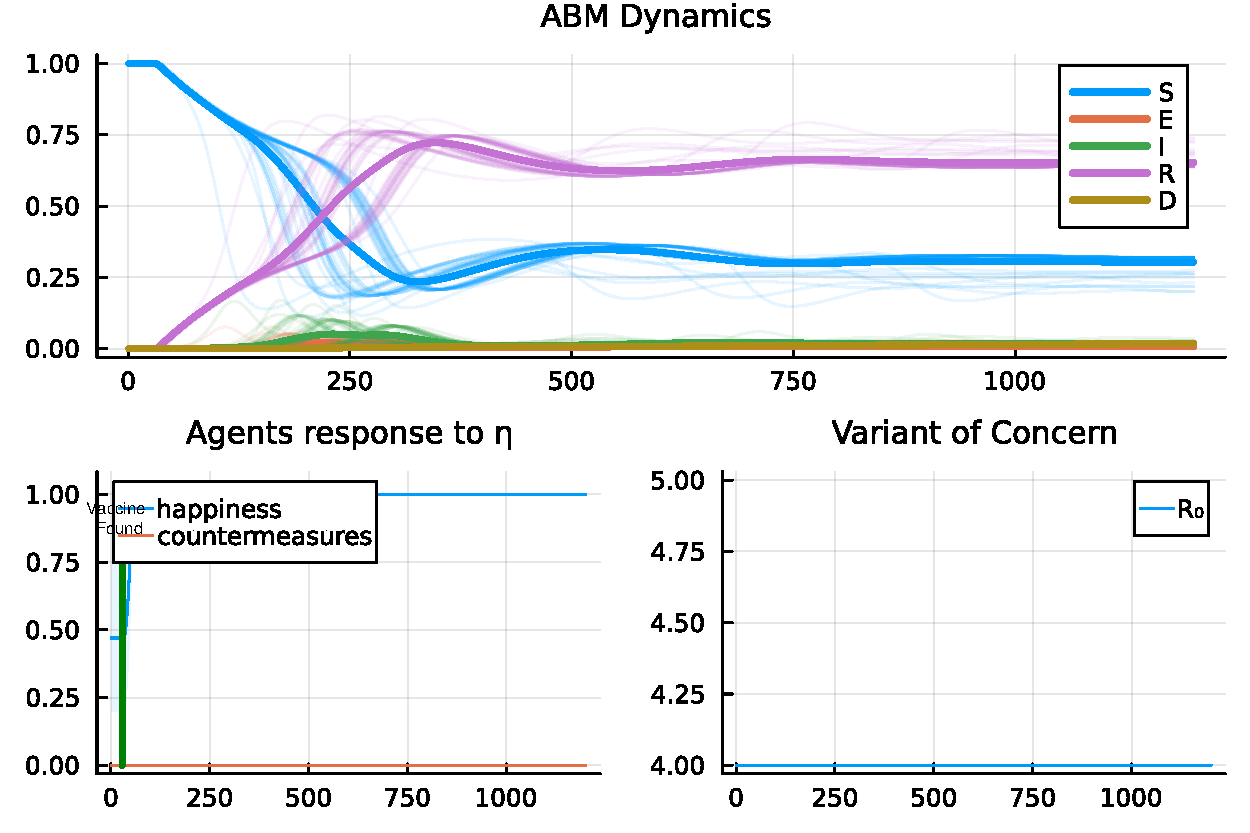
\includegraphics[width=\textwidth]{img/SocialNetworkABM_4_V.pdf}
		\caption{Grafico per la comparazione sul periodo di inizio della campagna vaccinale. Immediata}
		\label{fig:comparison_vax_1}
	\end{subfigure}
	\hfill
	\begin{subfigure}[b]{0.45\textwidth}
		\centering
		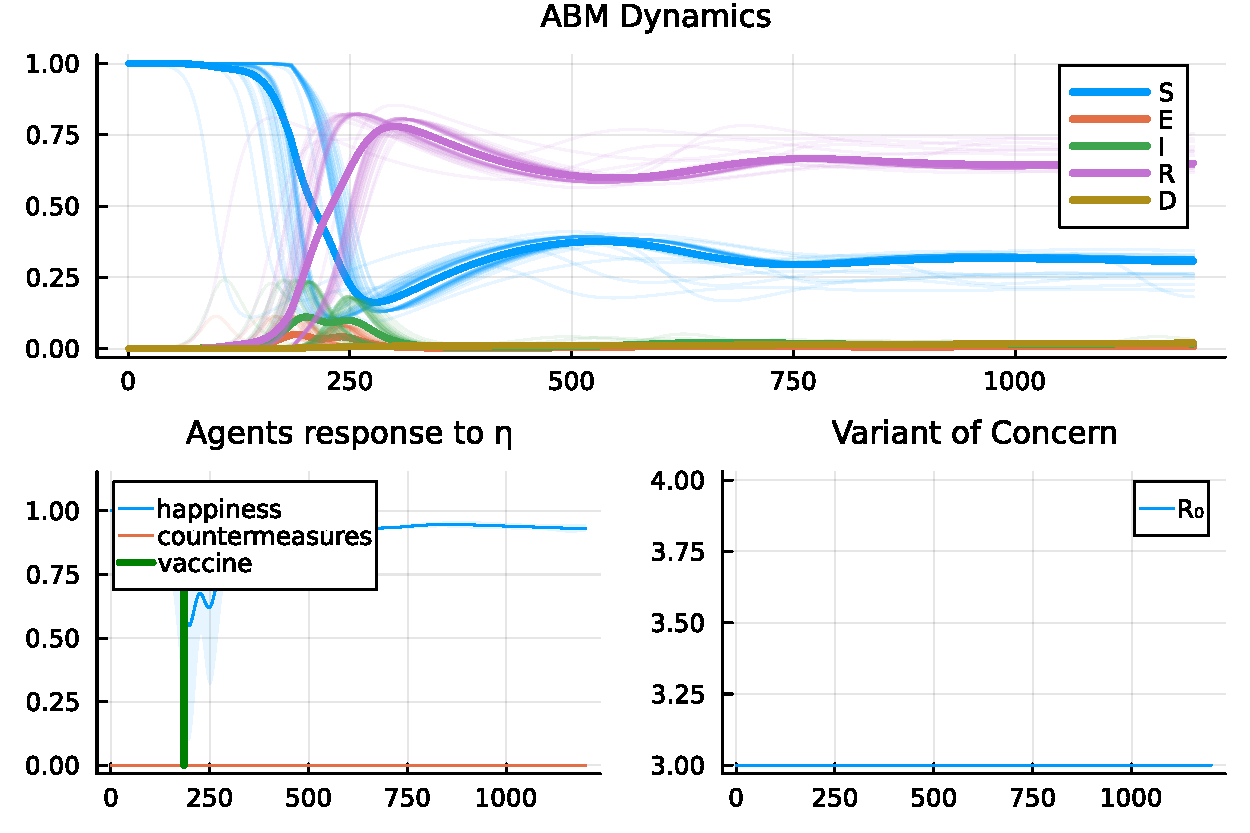
\includegraphics[width=\textwidth]{img/SocialNetworkABM_3_V.pdf}
		\caption{Grafico per la comparazione sul periodo di inizio della campagna vaccinale. Durante prima ondata}
		\label{fig:comparison_vax_2}
	\end{subfigure}
	\hfill
	\begin{subfigure}[b]{0.45\textwidth}
		\centering
		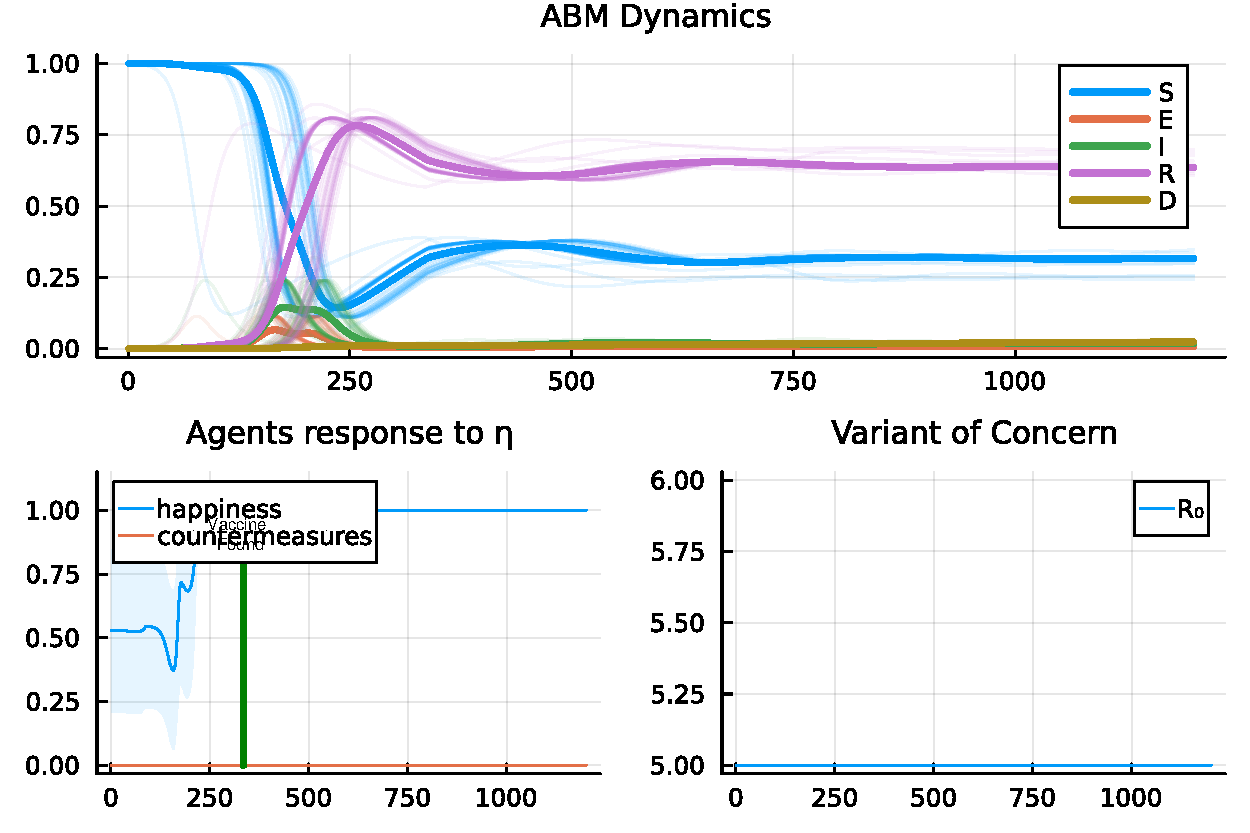
\includegraphics[width=\textwidth]{img/SocialNetworkABM_5_V.pdf}
		\caption{Grafico per la comparazione sul periodo di inizio della campagna vaccinale. Poco dopo la prima ondata}
		\label{fig:comparison_vax_3}
	\end{subfigure}
	\hfill
	\begin{subfigure}[b]{0.45\textwidth}
		\centering
		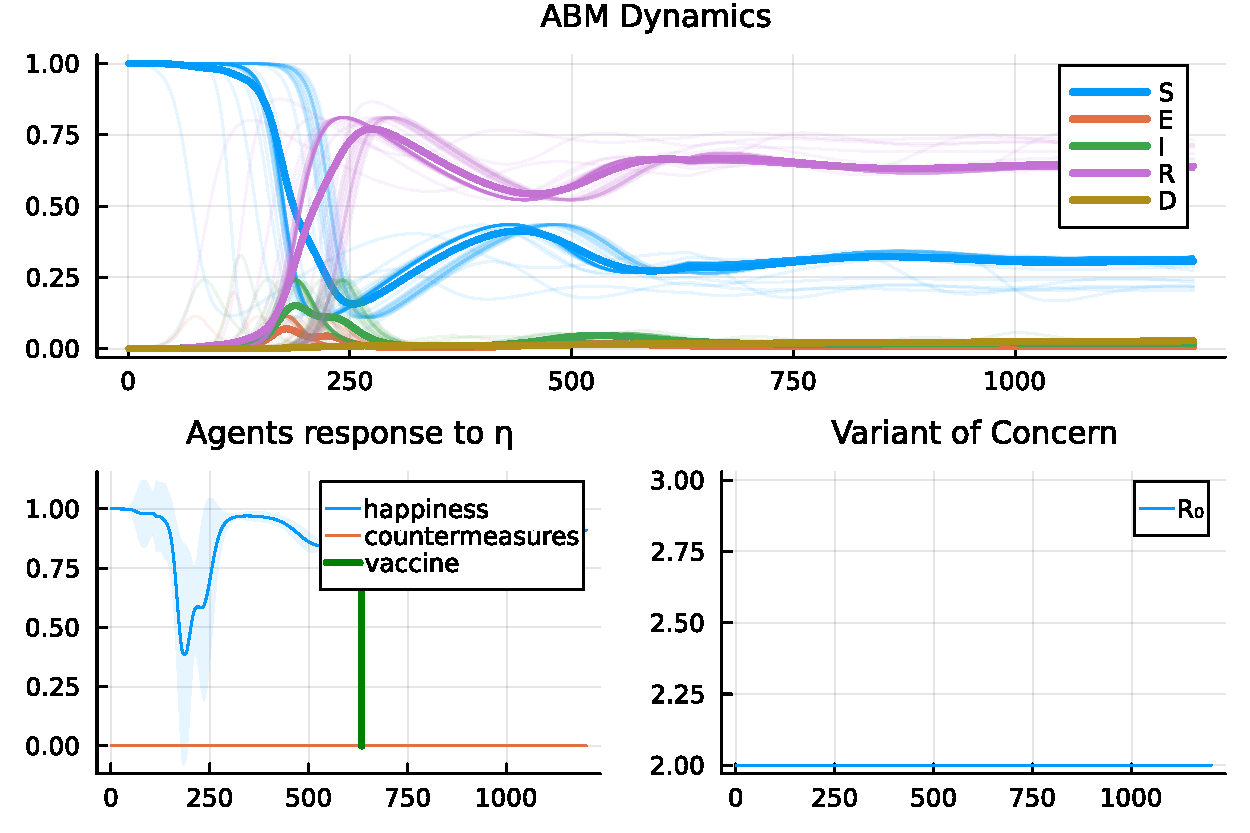
\includegraphics[width=\textwidth]{img/SocialNetworkABM_2_V.pdf}
		\caption{Grafico per la comparazione sul periodo di inizio della campagna vaccinale. In ritardo}
		\label{fig:comparison_vax_4}
	\end{subfigure}
\end{figure}

Questa visione semplicistica comunque è efficace nel modellare il decorso degli 
interventi farmaceutici per le contromisure contro una specifica epidemia, 
mostrando come l'applicazione di un vaccino e quindi la sua efficacia dipenda 
principalmente da quando inizia la campagna vaccinale, oltre che 
dal numero di persone a cui viene somministrato.